%========================================================================================%
%					NOTE
%========================================================================================%
% Probably this theme will not compile with standard pdftolatex compiler due to lack of some 
% fonts used in the theme. It is recommended to compile with XeLaTex instead.

% !TEX program = xelatex

%========================================================================================%
%					DOCUMENT SETUP
%========================================================================================%
\documentclass{beamer} 
\usetheme[progressbar=frametitle]{metropolis}

\usepackage{textpos}

\usepackage{amsmath}

\usepackage{mathrsfs}


%For making diagram and drawing
% \usepackage{tikz}
% \usetikzlibrary{shapes,arrows, fit, positioning}

%For appendix
\usepackage{appendixnumberbeamer}


\usepackage[export]{adjustbox}

%Some additional graphcs tools
%\usepackage{graphicx}
%\usepackage{datatool}
%\usepackage{animate}

% For someone using the pgfplot tools
%\usepackage{pgfplots}
%\usepgfplotslibrary{dateplot, groupplots}
%\pgfplotsset{compat=1.14}
%\usepgfplotslibrary{fillbetween}

%Remove words break, wrap instead
\usepackage[none]{hyphenat}


%for custom date
\usepackage[english]{babel}
\usepackage[nodayofweek,level]{datetime}

\usepackage{xspace}
\newcommand{\themename}{\textbf{\textsc{metropolis}}\xspace}

\renewcommand*{\arraystretch}{1.2}

\usefonttheme[onlymath]{serif}




%===================================================================================%
%				FRONT PAGE
%===================================================================================%
\titlegraphic{%
\hfill%

\includegraphics[height=1.5cm, valign=c]{logos/ccfd3.png}%
\hspace{15pt}%

\includegraphics[height=1.5cm, valign=c]{logos/symbol-PL.pdf}%
}

\author{MScEng Jakub Gałecki \\Thesis supervisor: ProfTit DSc Eng. Jacek Szumbarski} 

\title{Adjoint-Based Optimal Control of  Incompressible Flows with Open Boundary Conditions}

\institute{\textbf{Institute of Thermal Technology, Silesian University of Technology}}

\date{\vspace{5pt}\today}
% \date{\vspace{5pt}\formatdate{28}{9}{2017}}

%===================================================================================%
%				THEME COLORS
%===================================================================================%
% specify main colors which are being used by the theme
\definecolor{bordercolor}{HTML}{002699}
\definecolor{fillcolor}{HTML}{002699}

% fix theme black color which affects tikz plots
\definecolor{black}{RGB}{0,0,0}




%===================================================================================%
%				ACTUAL DOCUMENT CONTENT
%===================================================================================%

\begin{document}

\maketitle

%force to add logos to the each frame title
\addtobeamertemplate{frametitle}{}{%
\begin{textblock*}{100mm}(.9\textwidth,-0.9cm)
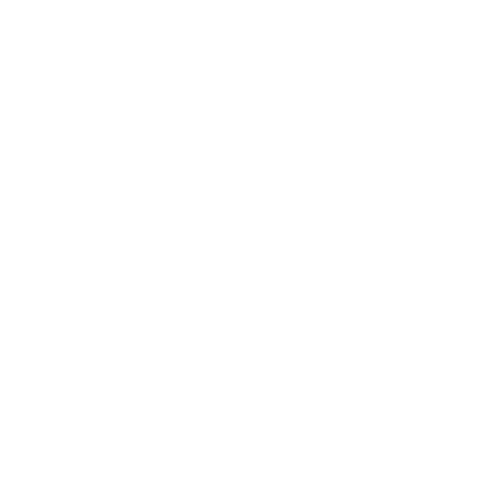
\includegraphics[height=0.8cm, valign=c]{logos/ccfd3_white.png}\hspace{10pt}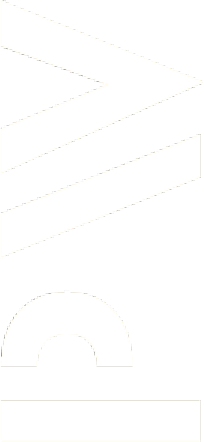
\includegraphics[height=0.78cm, valign=c]{logos/symbol-PL-white.pdf}
\end{textblock*}}

\begin{frame}{Agenda}

	\begin{itemize}
		\setlength\itemsep{1.5em}
		\item Open Boundary Conditions
		\begin{itemize}
			\item Pseudo-Traction Conditions
			\item Energy-Stable OBCs
			\item Open Dissipative BCs
		\end{itemize}
		\item Continuous Adjoint Method
		\item Solver Presentation
		\item Numerical Results
		\begin{itemize}
			\item Impinging Jet in Severely Truncated Domain
			\item Optimal Flow Rate Control in T-shaped Junction
		\end{itemize}
		\item Summary
	\end{itemize}
	
\end{frame}

% \section{Open Boundary Conditions}
\begin{frame}[standout]

    Open Boundary Conditions
	
\end{frame}

\begin{frame}{Governing equations}

	\metroset{block=fill}
	\begin{block}{Incompressible Navier-Stokes equations}
		\begin{equation}
			\begin{array}{cl}\left\{
				\begin{array}{c}
					\frac{\partial\mathbf{u}}{\partial t}+\left(\mathbf{u}\cdot\nabla\right)\mathbf{u}=-\nabla p+\nu\Delta\mathbf{u}+\mathbf{f}\\
					\nabla\cdot\mathbf{u}=0
				\end{array}\right. & in\;\Omega\\
			\mathbf{u}=\mathbf{u}_{D} & on\;\Gamma_{D}\\
			p\mathbf{n}-\nu\mathbf{n}\cdot\nabla\mathbf{u}-\mathbf{B}\left(\mathbf{u}\right)=f_{b}\left(t\right)\mathbf{n} & on\;\Gamma_{O}
			\end{array}
		\end{equation}
	\end{block}
	\begin{figure}
		\includegraphics[width=0.6\paperwidth]{pics/artificial_truncation_concept}
	\end{figure}

\end{frame}

\begin{frame}{Pseudo-traction conditions}

	\metroset{block=fill}
	\begin{block}{The pseudo-traction condition}
		\begin{equation}
			\mathbf{n}\cdot\mathbf{T}=p\mathbf{n}-\nu\mathbf{n}\cdot\nabla\mathbf{u}=P\left(t\right)\mathbf{n}
		\end{equation}
	\end{block}
	No outlet artifacts:
	\begin{figure}
		\includegraphics[width=0.9\paperwidth]{pics/pseudo_t_noart.jpg}
		Stokes flow around a cylinder in a channel
	\end{figure}

\end{frame}

\begin{frame}{Backflow instability}

	Unfortunately, especially at higher Reynolds numbers, the pseudo-traction condition suffers from backflow instability. Before we explain the cause of this phenomenon, let us see it in practice. Consider the following case:
	\begin{figure}
		\includegraphics[width=0.5\paperwidth]{pics/impinging_jet_setup.jpg}
	\end{figure}
	
\end{frame}

\begin{frame}{Backflow instability}

\alert{Let's have a look at the video to see what happens...}

\end{frame}

\begin{frame}{Backflow instability}

	\begin{figure}
		\includegraphics[width=0.6\paperwidth]{pics/velocity_tongues.jpg}
	\end{figure}

\end{frame}

\begin{frame}{Backflow instability}

	\begin{figure}
		\includegraphics[width=0.6\paperwidth]{pics/vorticity_tongues.jpg}
	\end{figure}

\end{frame}

\begin{frame}{Energy balance of the Navier-Stokes system}

	\metroset{block=fill}
	\begin{block}{Energy balance}
		\begin{multline}
			\frac{\partial}{\partial t}\int_{\Omega}\frac{1}{2}\left|\mathbf{u}\right|^{2}=-\nu\int_{\Omega}\left\Vert \nabla\mathbf{u}\right\Vert^{2}+\int_{\Omega}\mathbf{f}\cdot\mathbf{u}\,+ \\
			+\int_{\partial\Omega}\left(-p\mathbf{n}+\nu\mathbf{n}\cdot\nabla\mathbf{u}-\frac{1}{2}\left|\mathbf{u}\right|^{2}\mathbf{n}\right)\mathbf{u}
		\end{multline}
	\end{block}
	Stability problems stem from the presence of the $\frac{1}{2}\left|\mathbf{u}\right|^{2}\left(\mathbf{u}\cdot\mathbf{n}\right)$ term.
	
\end{frame}

\begin{frame}{Energy-stable OBCs}

	\metroset{block=fill}
	\begin{block}{Energy-stable open boundary condition}
		\begin{equation}
			p\mathbf{n}-\nu\mathbf{n}\cdot\nabla\mathbf{u}+\frac{1}{2}\Theta_{0}\left(\mathbf{u}\cdot\mathbf{n}\right)\left[\left|\mathbf{u}\right|^{2}\mathbf{n}+\left(\mathbf{u}\cdot\mathbf{n}\right)\mathbf{u}\right]=P\left(t\right)\mathbf{n}
		\end{equation}
	\end{block}
	where $\Theta_{0}$ is a smoothed step function:
	\begin{equation*}
		\Theta_{0}\left(\mathbf{u}\cdot\mathbf{n}\right)=\frac{1}{2}\left[1-\mathrm{tanh}\left(\frac{\mathbf{u}\cdot\mathbf{n}}{\delta U_{0}}\right)\right]
	\end{equation*}
	As $\delta\rightarrow 0$, the energy flux through the boundary where this BC is imposed becomes:
	\begin{equation}
			\Phi_{E}= \int_{\Gamma_{O}} - P \left( t \right) \left( \mathbf{n} \cdot \mathbf{u} \right) - \frac{1}{2} \left|\mathbf{u}\right|^{2} \left| \mathbf{n} \cdot \mathbf{u} \right|
	\end{equation}

\end{frame}

\begin{frame}{Open Dissipative BCs}

	\metroset{block=fill}
	\begin{block}{Open dissipative boundary condition}
		\begin{equation}
			p\mathbf{n}-\nu\mathbf{n}\cdot\nabla\mathbf{u}+\mathbf{n}\left[\left(\lambda+\gamma\frac{\partial}{\partial t}\right)\left(\mathbf{u}\cdot\mathbf{n}\right)+\chi\left|\mathbf{u}\cdot\mathbf{n}\right|\left(\mathbf{u}\cdot\mathbf{n}\right)\right]=P_{d}\left(t\right)\mathbf{n}
		\end{equation}
	\end{block}
	\begin{equation}
		P_{mean}=P_{d}+\left(\lambda+\gamma\frac{\mathrm{d}}{\mathrm{d}t}\right)\Phi+\chi\Phi\left|\Phi\right|
	\end{equation}
	\begin{figure}
		\includegraphics[width=0.8\paperwidth]{pics/od_concept.png}
		Conceptual illustration
	\end{figure}

\end{frame}

\begin{frame}[standout]
    Continuous Adjoint Method
\end{frame}

\begin{frame}{Optimal flow control}
Outline of the methodology:
\begin{itemize}
\item Define the objective functional to be minimized
\item Assume some initial design
\item Treat the flow problem as a "black box" input to some optimization procedure
\item Iterate until convergence (hopefully)
\end{itemize}
If we have can provide the optimization algorithm with information about the gradient of the objective functional w.r.t. the design variables, we can achieve drastically faster convergence. Computing this gradient is where things get tricky.
\end{frame}

\begin{frame}{The continuous adjoint method}
	
	\begin{itemize}
		% \setlength\itemsep{1em}
		\item Our goal: compute the gradient of some objective function/functional with regards to control variables
		\item Problem: treated naively, this problem requires computing the derivatives of the state variables w.r.t. the control variables
		\item The adjoint method allows us to circumvent this issue and compute the sensitivity of the objective functional directly
	\end{itemize}
	Let us consider an abstract problem, where the evolution of the state variable is given by
	\begin{equation}
		\left\{ \begin{array}{c}
		\frac{d\mathbf{u}}{dt}+\mathbf{\mathcal{N}}\left(\mathbf{u},\mathbf{q}\right)=0\\
		\left.\mathbf{u}\right|_{t=0}=\mathbf{u}_{0}
		\end{array}\right.
	\end{equation}
	
\end{frame}

\begin{frame}{The continuous adjoint method}

	Let us define the objective functional
	\begin{equation}
		\mathcal{J}=\int_{0}^{T} j\left(\mathbf{u},\mathbf{q}\right)\,\mathrm{d}t
	\end{equation}
	We introduce the augmented functional
	\begin{equation}
		\mathcal{H}=\int_{0}^{T} j\left(\mathbf{u},\mathbf{q}\right)\,\mathrm{d}t+\int_{0}^{T}\left(\mathbf{w},\frac{d\mathbf{u}}{dt}+\mathbf{\mathcal{N}}\left(\mathbf{u},\mathbf{q}\right)\right)_{\mathscr{U}}\,\mathrm{d}t
	\end{equation}
	Note that due to the state constraints
	\begin{equation}
		\mathcal{H}\equiv\mathcal{J}
	\end{equation}
	
\end{frame}

\begin{frame}{The continuous adjoint method}

	The first variation of the augmented functional reads
	\begin{multline}
		\delta\mathcal{H}=\int_{0}^{T}\left[\left(\delta\mathbf{u},\left(\frac{\partial}{\partial\mathbf{u}} j\right)\left(\mathbf{u},\mathbf{q}\right)\right)_{\mathscr{U}}+\left(\delta\mathbf{q},\left(\frac{\partial}{\partial\mathbf{q}} j\right)\left(\mathbf{u},\mathbf{q}\right)\right)_{\mathscr{Q}}\right]\,\mathrm{d}t+\\+\int_{0}^{T}\left(\mathbf{w},\frac{d\delta\mathbf{u}}{dt}+\delta\mathbf{u}\left(\frac{\partial}{\partial\mathbf{u}}\mathbf{\mathcal{N}}\right)\left(\mathbf{u},\mathbf{q}\right)+\delta\mathbf{q}\left(\frac{\partial}{\partial\mathbf{q}}\mathbf{\mathcal{N}}\right)\left(\mathbf{u},\mathbf{q}\right)\right)_{\mathscr{U}}\,\mathrm{d}t
	\end{multline}
	After some transformations, we arrive at
	\begin{multline}
		\delta\mathcal{H}=\int_{0}^{T}\left(\delta\mathbf{u},-\frac{d\mathbf{w}}{dt}+\left(\frac{\partial}{\partial\mathbf{u}}\mathbf{\mathcal{N}}\right)^{*}\left(\mathbf{u},\mathbf{q}\right)\mathbf{w}+\left(\frac{\partial}{\partial\mathbf{u}} j\right)\left(\mathbf{u},\mathbf{q}\right)\mathbf{u}\right)_{\mathscr{U}}\,\mathrm{d}t+\\+\int_{0}^{T}\left(\delta\mathbf{q},\left(\frac{\partial}{\partial\mathbf{q}}\mathbf{\mathcal{N}}\right)^{*}\left(\mathbf{u},\mathbf{q}\right)\mathbf{w}+\left(\frac{\partial}{\partial\mathbf{q}} j\right)\left(\mathbf{u},\mathbf{q}\right)\mathbf{q}\right)_{\mathscr{Q}}\,\mathrm{d}t+\left(\mathbf{w}\left(t\right),\delta\mathbf{u}\left(t\right)\right)_{\mathscr{U}}
	\end{multline}

\end{frame}

\begin{frame}{The continuous adjoint method}

	We can now write the adjoint equations
	\begin{equation}
		\left\{ \begin{array}{c}
		-\frac{d\mathbf{w}}{dt}+\left(\frac{\partial}{\partial\mathbf{u}}\mathbf{\mathcal{N}}\right)^{*}\left(\mathbf{u},\mathbf{q}\right)\mathbf{w}+\left(\frac{\partial}{\partial\mathbf{u}} j\right)\left(\mathbf{u},\mathbf{q}\right)\mathbf{u}=\mathbf{0}\\
		\left.\mathbf{w}\right|_{t=T}=\mathbf{0}
		\end{array}\right.
	\end{equation}
	And the objective function gradient at instant $t$ is given by
	\begin{equation}
		\left.\nabla_{\mathbf{q}}\mathcal{J}\left(\mathbf{u},\mathbf{q}\right)\right|_{t}=\left(\frac{\partial}{\partial\mathbf{q}}\mathbf{\mathcal{N}}\right)^{*}\left[\mathbf{u}\left(t\right),\mathbf{q}\left(t\right)\right]\mathbf{w}\left(t\right)+\left(\frac{\partial}{\partial\mathbf{q}} j\right)\left[\mathbf{u}\left(t\right),\mathbf{q}\left(t\right)\right]\mathbf{q}\left(t\right)
	\end{equation}

\end{frame}

\begin{frame}{Adjoint-based optimal flow control}
\metroset{block=fill}
\begin{block}{General algorithm}
\begin{enumerate}
\item Take initial design $\mathbf{q}_0$
\item Integrate flow problem in time based on $\mathbf{q}_n$, retain flow history
\item Integrate adjoint problem backwards in time
\item Compute $\nabla_{\mathbf{q}}\mathcal{J}\left(\mathbf{u},\mathbf{q}\right)$
\item Based on some optimization procedure, obtain $\mathbf{q}_{n + 1}$
\item Repeat steps 2-5 until convergence
\end{enumerate}
\end{block}
\end{frame}

\begin{frame}{Adjoint equations: flow rate control problem}

	Let us now take a look at the specific example of optimal flow rate control. Our state constraints take the form of the Navier-Stokes equations with appropriate boundary conditions (see first slide). We can define our objective functional as
	\begin{equation}
		\mathcal{J}=\frac{1}{2T}\int_{0}^{T}\sum_{i=0}^{k}\left[\int_{\Gamma_{i}}\mathbf{u}\cdot\mathbf{n}\,\mathrm{d}S-\Phi_{i}\left(t\right)\right]^{2}\,\mathrm{d}t
	\end{equation}
	where $\Phi_{i}$ denotes the desired flow rate through $\Gamma_{i}$

\end{frame}

\begin{frame}{Adjoint equations: flow rate control problem}

	The extended functional is
	\begin{multline}
		\mathcal{H}=\mathcal{J}+\int_{0}^{T}\int_{\Omega}\left[\frac{\partial\mathbf{u}}{\partial t}+\left(\mathbf{u}\cdot\nabla\right)\mathbf{u}+\nabla p-\nu\Delta\mathbf{u}\right]\cdot\mathbf{w}\,\mathrm{d}\mathbf{x}\mathrm{d}t- \\
		-\int_{0}^{T}\int_{\Omega}\left(\nabla\cdot\mathbf{u}\right)s\,\mathrm{d}\mathbf{x}\mathrm{d}t
	\end{multline}
	Let's look at the variation of its individual components
	\begin{equation}
		\delta\mathcal{J}=\int_{0}^{T}\sum_{i=0}^{k}\frac{1}{T}\left[\int_{\Gamma_{i}}\mathbf{u}\cdot\mathbf{n}\,\mathrm{d}S-\Phi_{i}\left(t\right)\right]\mathbf{n}\cdot\delta\mathbf{u}\,\mathrm{d}t
	\end{equation}

\end{frame}

\begin{frame}{Adjoint equations: flow rate control problem}

	The variation of the remaining components can be written as
	\begin{multline}
		\delta\mathcal{I}_{NS}=\int_{0}^{T}\int_{\Omega}\left[\frac{\partial\left(\delta\mathbf{u}\right)}{\partial t}+\left(\mathbf{u}\cdot\nabla\right)\delta\mathbf{u}+\left(\delta\mathbf{u}\cdot\nabla\right)\mathbf{u}\right]\cdot\mathbf{w}\,\mathrm{d}\mathbf{x}\mathrm{d}t+\\
		+\int_{0}^{T}\int_{\Omega}\left[\nabla\left(\delta p\right)-\nu\Delta\left(\delta\mathbf{u}\right)\right]\cdot\mathbf{w}\,\mathrm{d}\mathbf{x}\mathrm{d}t-\\
		-\int_{0}^{T}\int_{\Omega}\left(\nabla\cdot\delta\mathbf{u}\right)s\,\mathrm{d}\mathbf{x}\mathrm{d}t
	\end{multline}

\end{frame}

\begin{frame}{Adjoint equations: flow rate control problem}

	After some laborious transformations, we arrive at the equation
	\begin{multline}
		\delta\mathcal{I}_{NS}=\int_{\Omega}\mathbf{w}(T)\cdot\delta\mathbf{u}\left(T\right)\,\mathrm{d}\mathbf{x}+\\
		+\int_{0}^{T}\int_{\Omega}\left[-\frac{\partial\mathbf{w}}{\partial t}-\left(\mathbf{u}\cdot\nabla\right)\mathbf{w}+\left(\nabla\mathbf{u}\right)^{T}\cdot\mathbf{w}-\nu\Delta\mathbf{w}+\nabla s\right]\cdot\delta\mathbf{u}\,\mathrm{d}\mathbf{x}\mathrm{d}t+\\
		+\int_{0}^{T}\int_{\Omega}(-\nabla\cdot\mathbf{w})\delta p\,\mathrm{d}\mathbf{x}\mathrm{d}t+\\
		+\int_{0}^{T}\int_{\partial\Omega}\left[\left(\mathbf{u}\cdot\mathbf{n}\right)\mathbf{w}+\nu\frac{\partial\mathbf{w}}{\partial\mathbf{n}}-s\mathbf{n}\right]\cdot\delta\mathbf{u}\,\mathrm{d}S\mathrm{d}t+\\
		+\int_{0}^{T}\int_{\partial\Omega}\left[\mathbf{w}\cdot\mathbf{n}\delta p-\nu\frac{\partial\left(\delta\mathbf{u}\right)}{\partial\mathbf{n}}\cdot\mathbf{w}\right]\,\mathrm{d}S\mathrm{d}t
	\end{multline}

\end{frame}

\begin{frame}{Adjoint equations: flow rate control problem}
	
	In order for the variation of the state variables to disappear in the domain, the following equations must hold
	\begin{equation}
		\left\{ \begin{array}{c}
		-\frac{\partial\mathbf{w}}{\partial t}-\left(\mathbf{u}\cdot\nabla\right)\mathbf{w}+\left(\nabla\mathbf{u}\right)^{T}\mathbf{w}=-\nabla s+\nu\Delta\mathbf{w}\\
		\nabla\cdot\mathbf{w}=0
		\end{array}\right.\quad in\:\Omega
	\end{equation}
	The terminal condition is
	\begin{equation}
		\left.\mathbf{w}\right|_{t=T}=\mathbf{0}
	\end{equation}
	All that is left is to formulate appropriate boundary conditions
	
\end{frame}

\begin{frame}{Adjoint equations: flow rate control problem}

	Without much difficulty, we can show that if we are able to construct a function $\mathbf{b}\left(\mathbf{u},\mathbf{w}\right)$ such that
	\begin{equation}
		\mathbf{w}\cdot\delta\mathbf{B}\left(\mathbf{u}\right)=\mathbf{b}\left(\mathbf{u},\mathbf{w}\right)\delta\mathbf{u}
	\end{equation}
	then the boundary condition for the adjoint field becomes
	\begin{multline}
		s\mathbf{n}-\left(\mathbf{u}\cdot\mathbf{n}\right)\mathbf{w}-\nu\frac{\partial\mathbf{w}}{\partial\mathbf{n}}-\mathbf{b}\left(\mathbf{u},\mathbf{w}\right)=\\
		=\frac{1}{T}\left[\int_{\Gamma_{i}}\mathbf{u}\cdot\mathbf{n}\,\mathrm{d}S-\Phi_{i}\left(t\right)\right]\mathbf{n}\quad on\:\Gamma_{O}
	\end{multline}
	The construction of such a function is again very laborious, and we only quote the results.

\end{frame}

\begin{frame}{Adjoint equations: flow rate control problem}

	For the trivial case of the pseudo-traction conditions, we have
	\begin{equation}
		\mathbf{b}\equiv\mathbf{0}
	\end{equation}
	For the open dissipative conditions:
	\begin{equation}
		\mathbf{b}=\mathbf{n}\left[\left(\lambda-\gamma\frac{\partial}{\partial t}\right)\left(\mathbf{w}\cdot\mathbf{n}\right)+2\chi\left|\mathbf{u}\cdot\mathbf{n}\right|\left(\mathbf{w}\cdot\mathbf{n}\right)\right]
	\end{equation}
	Finally, for the energy-stable BCs:
	\begin{multline}
		\mathbf{b}=\frac{1}{4}\left\{ \vphantom{{\left[\left|\mathbf{u}\right|^{2}\left(\mathbf{n}\cdot\mathbf{w}\right)+\left(\mathbf{n}\cdot\mathbf{u}\right)\left(\mathbf{u}\cdot\mathbf{w}\right)\right]\frac{\mathbf{n}}{\mathrm{cosh}^{2}\left(\frac{\mathbf{n}\cdot\mathbf{u}}{U_{0}\cdot\delta_{s}}\right)U_{0}\cdot\delta_{s}}}}\left[1-\mathrm{tanh}\left(\frac{\mathbf{u}\cdot\mathbf{n}}{U_{0}\delta_{s}}\right)\right]\left[2\mathbf{u}\left(\mathbf{n}\cdot\mathbf{w}\right)+\mathbf{n}\left(\mathbf{u}\cdot\mathbf{w}\right)+\left(\mathbf{n}\cdot\mathbf{u}\right)\mathbf{w}\right]\right.+\\
		+\left.\left[\left|\mathbf{u}\right|^{2}\left(\mathbf{n}\cdot\mathbf{w}\right)+\left(\mathbf{n}\cdot\mathbf{u}\right)\left(\mathbf{u}\cdot\mathbf{w}\right)\right]\frac{\mathbf{n}}{\mathrm{cosh}^{2}\left(\frac{\mathbf{n}\cdot\mathbf{u}}{U_{0}\cdot\delta_{s}}\right)U_{0}{\color{orange}\delta_{s}}}\right\} 
	\end{multline}

\end{frame}

\begin{frame}{Adjoint equations: flow rate control problem}

	Finally, we can express the gradient of the objective functional with respect to the boundary pressures $P_{i}$ with the surprisingly elegant formula
	\begin{equation}
		\nabla_{P_{i}}\mathcal{J}=\int_{\Gamma_{i}}\mathbf{w}\cdot\mathbf{n}\,\mathrm{d}S
	\end{equation}

\end{frame}

\begin{frame}[standout]
    Solver presentation
\end{frame}

\begin{frame}{Flow solver}
	
	\begin{itemize}
		\setlength\itemsep{1em}
		\item \alert{Formulation:} Least-squares (finite element)
		\item \alert{Spatial discretization:} Quadrilateral spectral elements (Lobatto nodal base)
		\item \alert{Temporal discretization:} BDF2 (for both the primal and adjoint solvers)
		\item \alert{Convective term linearization:} Newton's method
		\item \alert{Numerical integration:} Full order Gauss-Legendre quadrature
		\item \alert{Algebraic solver:} Sparse LU solver
	\end{itemize}
	
\end{frame}

\begin{frame}{Optimization solver}
	
	\begin{itemize}
		\item MATLAB Optimization Toolbox: nonlinear unconstrained minimization (fminunc)
		\item Quasi-Newton algorithm with BFGS Hessian update		
	\end{itemize}
	Search direction:
	\begin{equation*}
		\mathbf{d}_{i}=-\mathbf{H}_{i}^{-1}\nabla_{\mathbf{q}}\mathcal{J}\left(\mathbf{u},\mathbf{q}_{i}\right)
	\end{equation*}
	Hessian update:
	\begin{equation*}
		\mathbf{H}_{i+1}=\mathbf{H}_{i}+\frac{\mathbf{g}_{i}\mathbf{g}_{i}^{T}}{\mathbf{g}_{i}\mathbf{s}_{i}}-\frac{\mathbf{H}_{i}\mathbf{s}_{i}\mathbf{s}_{i}^{T}\mathbf{H}_{i}^{T}}{\mathbf{s}_{i}^{T}\mathbf{H}_{i}\mathbf{s}_{i}}
	\end{equation*}
	
\end{frame}

\begin{frame}[standout]
    Numerical results
\end{frame}

\begin{frame}{Impinging jet in a severely truncated domain}
	
	We recall the problem previously used to demonstrate backflow instability:
	\begin{figure}
		\includegraphics[width=0.5\paperwidth]{pics/impinging_jet_setup.jpg}
	\end{figure}
	This time we impose the Energy-stable OBCs

\end{frame}

\begin{frame}{Impinging jet in a severely truncated domain}

	\begin{figure}
		\includegraphics[width=0.7\paperwidth]{pics/x_vel_stable.jpg}
	\end{figure}

\end{frame}

\begin{frame}{Impinging jet in a severely truncated domain}

	\begin{figure}
		\includegraphics[width=0.7\paperwidth]{pics/vort_stable.jpg}
	\end{figure}

\end{frame}

\begin{frame}{Optimal flow rate control in T-shaped junction}

	\begin{figure}
		\includegraphics[width=0.7\paperwidth]{pics/geo_mesh.eps}
	\end{figure}

\end{frame}

\begin{frame}{Optimal flow rate control in T-shaped junction}

	\begin{itemize}
		\setlength\itemsep{0.5em}
		\item Parabolic inlet velocity profile
		\item No-slip walls
		\item Open boundary conditions at the outlets (3 separate problems corresponding to the 3 different types of OBCs presented)
		\item Pressure value at right outlet prescribed as:
	\end{itemize}
	\begin{equation*}
		P\left(t\right)=8t\mathrm{sin}\left(2\pi t\right)
	\end{equation*}

\end{frame}

\begin{frame}{Results at $Re=20$, pseudo-traction conditions}

	\begin{figure}
		\includegraphics[width=0.85\paperwidth]{pics/Re_20_conv.eps}
	\end{figure}

\end{frame}

\begin{frame}{Results at $Re=20$, pseudo-traction conditions}

	\begin{figure}
		\includegraphics[width=0.85\paperwidth]{pics/Re_20_sol.eps}
	\end{figure}

\end{frame}

\begin{frame}{Results at $Re=50$, open dissipative conditions}

	\begin{figure}
		\includegraphics[width=0.85\paperwidth]{pics/Re50_conv.eps}
	\end{figure}

\end{frame}

\begin{frame}{Results at $Re=50$, open dissipative conditions}

	\begin{figure}
		\includegraphics[width=0.85\paperwidth]{pics/Re50_sol.eps}
	\end{figure}

\end{frame}

\begin{frame}{Results at $Re=500$, energy-stable conditions}

	\begin{figure}
		\includegraphics[width=0.85\paperwidth]{pics/Re500_conv.eps}
	\end{figure}

\end{frame}

\begin{frame}{Results at $Re=500$, energy-stable conditions}

	\begin{figure}
		\includegraphics[width=0.85\paperwidth]{pics/Re500_sol.eps}
	\end{figure}

\end{frame}

\begin{frame}{Summary of accomplishments}

\begin{itemize}

	\item Implementation of a LSSEM-based flow solver
	\item Implementation of open boundary conditions within this framework
	\begin{itemize}
		\item pseudo-traction
		\item energy-stable*
		\item open dissipative*
	\end{itemize}
	\item Implementation of a LSSEM-based adjoint solver
	\item Derivation of adjoint equations for ESOBCs*
	\item Numerical verification of the proposed optimal flow control approach
	

\end{itemize}

\end{frame}

\appendix

\begin{frame}{Q\&A}
    \alert{Thank you for listening}
\end{frame}

\end{document}
